\documentclass[notitlepage,12pt]{report}
\usepackage[left=0.5in, right=0.5in, top=0.5in, bottom=0.5in]{geometry}

\usepackage{titling}
\usepackage{lipsum}
\usepackage{braket}
\usepackage{graphicx}
\usepackage[table]{xcolor}
\graphicspath{./images/}
\usepackage{subcaption}
\newcommand{\tr}{\mathrm{tr}}
\usepackage{hyperref}
\usepackage{authblk}
\usepackage[backend=biber, style=chem-acs]{biblatex}
\usepackage{tabularx}
% \usepackage{amsmath}
\usepackage{mathtools}% Loads amsmath
\usepackage{physics}
\usepackage{wrapfig}
\renewcommand\thesection{\arabic{section}}

\bibliography{bib}
\addbibresource{bib.bib}

\def\br{{\mathbf{r}}}
\def\bG{{\mathbf{G}}}
\def\brp{{\mathbf{r}^\prime}}


\begin{document}
%	\title{Electronic properties in condensed-phase molecular systems under Embedded theoretical approaches: Liquid water systems}
%	\author[1]{Jessica Martinez}
%	\affil[1]{Department of Chemistry, Rutgers University, Newark, New Jersey}
%	\date{June 2022}
	\renewcommand\Affilfont{\itshape\small}
%	\thispagestyle{empty}
%\maketitle
\begin{center}
    \textbf{\LARGE Accurate models of molecular bulk systems from first principles}\\
    Jessica Martinez, Rutgers University-Newark
\end{center}
\section{Motivations and scientific basis for the collaboration}

    The Pavanello and Gomes groups develop electronic structure methods for the in-silico prediction of molecular and materials properties. The two groups have been collaborating since 2017 and the collaboration so far produced one journal article \supercite{tolle2019charged} and resulted in training of 3 Rutgers-based PhD students and the development of three software modules in the softwares embedded Quantum ESPRESSO \supercite{}, DIRAC \supercite{}, and PyADF \supercite{}. The collaboration has been fuelled by two visits of Prof Gomes to Rutgers in 2014 and 2016. Unfortunately, the past two years have been negatively affected by the COVID pandemic and any international travel was forbidden. 

    Since joining Rutgers as a PhD student in 2019, I have been working on applying the methds developed by the collaboration which embed molecular  electronic structures in density functional environments (DFT embedding) to determine the ionization potential of water and dissect its dependence on order parameters of the liquid (e.g., the instantaneous structure of  the liquid surrounding a particular molecule that is being ionized).  With the Chateauxbriand fellowship, I will be able to travel to Prof Gomes's lab and not only extend the current method to include accurate his most recent wavefunction methods based on equation of motion coupled cluster in DFT environments but also to implement completely new electronic structure methods. I will then apply the methods to shed light on timely and important questions related to the electron and nuclear dynamics following an ionization or an X-Ray absorption in condensed phases. Such questions are particularly timely given the several novel experimental techniques based on facility-based free electron lasers that probe electron dynamics at the attosecond timescale \supercite{}.  

    The accurate description of processes occurring in condensed-phase molecular systems requires a symbiotic  equilibrium between spectroscopic techniques\supercite{reimann2021two,malerz2021low,bolognesi2021combined} and computational approaches \supercite{couto2007understanding,ambrosio2016structural,ozaki2021advances}. For example, photoelectron spectroscopy \supercite{thurmer2021accurate,perry2020ionization,credidio2021quantitative,thurmer2021valence,tolle2019charged,gaiduk2018electron,gaiduk2016photoelectron,seidel2016valence} and X-Ray absorption spectroscopy (XAS)\supercite{zhovtobriukh2019liquid,zhang2020isotope,smith2020femtosecond} are among those experimental characterization techniques that routinely rely on computational methods for the resolution of the spectra or their interpretation.
	
    In-depth knowledge of the factors influencing, e.g., the ionization potential (IP) of liquid water could allow the control and better understanding of many crucial processes in electrochemistry\supercite{marenich2014computational}, photochemistry\supercite{reuther1996primary,hu2021photochemical} as well as peculiar states of matter like excess electrons solvated in liquid water\supercite{ambrosio2017electronic}.  Recent advances in liquid microjet  photoelectron spectroscopy have opened the door to the determination of accurate electronic energetics of water and aqueous solutions \supercite{thurmer2021accurate,perry2020ionization,credidio2021quantitative,thurmer2021valence} deliverng the  most accurate value for the IP of liquid water, 11.33 $\pm$0.03 eV. 

    Such advances have, in turn, prompted simulations to provide an equally accurate description of ionization usgin electronic structure techniques, such as GW based on periodic pseudopotential DFT \supercite{gaiduk2018electron,ziaei2018probing,dal2014pseudopotentials} delivering excellent agreement with the experiment.
	
    Along similar lines of research, the {\bf Pavanello and Gomes groups} recently developed a method which we call ``impurity model'' based on subsystem DFT \supercite{jacob2014subsystem,wesolowski2015frozen,krishtal2015subsystem} for computing ionization energies (both electron attachment and detachment) of bulk molecular systems \supercite{tolle2019charged}. In subsystem DFT,  the total electron density, $\rho(\br)$ is divided into a sum of subsystem densities 
\begin{equation}
    \label{dens}
    \rho(\br) = \sum_I^{N_S}\rho_I(\br)
\end{equation}
    where $N_S$ is the number of independent subsystems in the simulation and the subsystems are identified by each molecule. The subsystem electron densities are determined by a variational procedure which imposes the total energy functional to be stationary wrt variations of each subsystem density. The core of the impurity model is that a $\Delta$SCF procedure\supercite{bagus1965self,waskom2017mwaskom} can be used to compute ionization energies, for the IP we use $IP=E^+-E^0$ where $E^{+/0}$ is the total energy of the ionized/neutral system. The main issue arises when employing periodic boundary conditions (which is the most common method for approaching bulk systems with atomistic models) because a charged system has an infinite energy due to the self-interaction of the excess charge between the infinite number of periodic images. The impurity model solves this problem by subdividin the subsystems into two categories: (1) finite subsystems, whose Coulomb potential is given by the nonperiodic potential (i.e., $v[\rho^{\text{finite}}](\br)=\int\frac{\rho^{\text{finite}}(\brp)}{|\brp-\br|}d\brp$); (2) extended subsystems, whose potential is given by the fully periodic one (i.e., in reciprocal space, $\tilde v[\rho^{\text{extended}}](\bG)=\frac{4\pi}{|\bG|^2}\tilde\rho^\text{extended}(\bG)$ where the tildas imply Fourier transform).

    The subsystem DFT description of the electronic structure allowed us to break down the IP of liquid water  into five energy contributions:  {\bf (1)} Mean field: the ionization energy of each water molecule computed at Hartree-Fock level; {\bf (2)} Correlation: electron correlation within each water molecule at the correlated wavefunction level as well as DFT; {\bf (3)} Embeddingnd: Coulomb interactions between each water molecule and their environment augmented by effects of exchange, correlation and Pauli repulsion; {\bf (4)} Polarization: polarization of the environment electronic structure in response to the ionization of a nearby water molecule; and finally, {\bf (5)} Delocalization: the possibility that the spin density of the cation is delocalized over more than one water molecule. By averaging results from  128  snapshots of a 64-molecule model of liquid water (in periodic boundary conditions) \supercite{gaiduk2018electron}, the five contributions were calculated and are summarized in Figure \ref{cont_ip} 
\begin{wrapfigure}{l}{0.4\textwidth}
	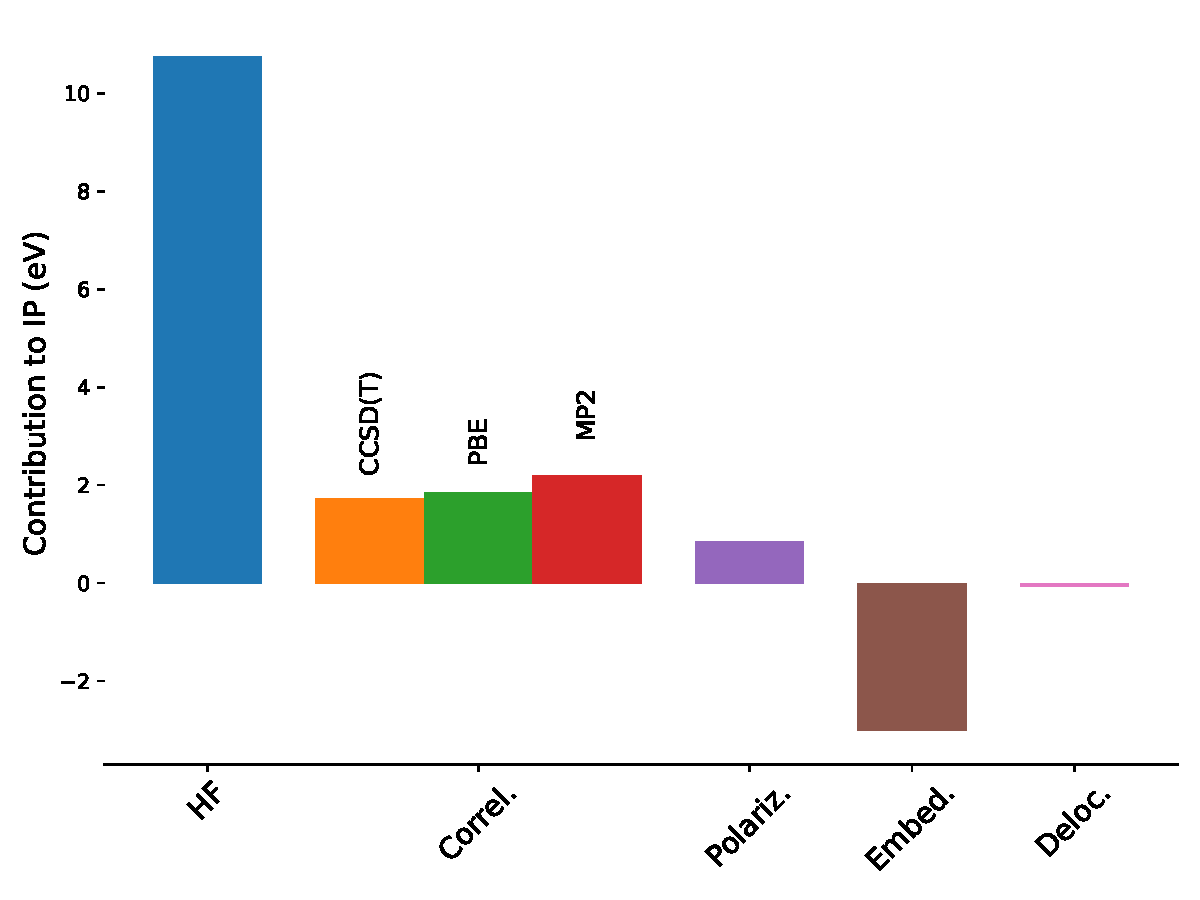
\includegraphics[width=\linewidth]{./images/contribution_liquidwater_PI}
    \caption{\label{cont_ip}Five contributions to the IP of water (see text). Their interplay highlights the complexity of the electronic processes occurring when water is ionized. \supercite{}}
\end{wrapfigure}
    The correlation contribution was calculated by DFT-embedded wavefunction methods such as CCSD(T) and MP2 as well as pure DFT functionals such as PBE and contributed by about 2 eV. The polarization of the electronic environment nearby an ionized water molecule contributes for about 0.84 eV while the embedding correction (i.e., the interaction with the environment) contributes negatively by 2.8 eV. Accounting for spin density delocalization over more than one water molecule contributed by a negligible amount. Such a granularity in the description of the ionization process is unprecedented and highlights the capabilities of the method developed by this collaboration. 	
	
    \section{Proposed work}
    With granted funding, the Chateaubriand fellowship will allow me to build upon the existing collaborative work to develop a comprehensive and accurate model of ionization {\bf and } core-electron excitation in molecular bulk systems. Leveraging the impurity model, I wish to combine the subsystem DFT and the real-time block-orthogonalized Manby-Miller embedding (BOMME) \supercite{ding2017embedded,koh2017accelerating} developed by the Gomes group to extend my analysis of the ionization processes in water to also model X-Ray absorption near-edge structures (XANES)\supercite{fransson2016x}. XANES allow the study of the oxidation state, local symmetry, and coordination environment in gas, liquid, and solid phases\supercite{rehr2005progress,koningsberger1987x}. 
    Particularly, for the simulation of X-Ray absorption spectroscopy in liquids, multiple theoretical approaches have been developed, such as transition potential (TP)-DFT \supercite{triguero1998calculations}, time-dependent DFT (TDDFT) employing Davidson procedure\supercite{davidson197514}, Excited-state core hole (XCH)\supercite{prendergast2006x}, GW \supercite{vinson2012theoretical,chen2010x}, and QM/MM techniques ased on TDDFT \supercite{list2014lanczos}. A detailed description of each approach is found in the review \cite{fransson2016x}.
	
	In this project, taking advantage of the newest implementation of rt-BOMME and rt-subsystem DFT \supercite{de2021environment} in the Psi4 code \supercite{smith2020psi4} by Gomes and collaborators, to predict and overcome the already mentioned failures in the modeling of the X-ray absorption near-edge structures (XANES), we wish to go further in applications of the method accounting for more than first solvation shells. To accomplish this, we selected three main thrusts of research (1) Liquid water and Ice, (2) Cations solvated in water, and (3) A complex molecule ($K_3[Fe(CN)_6]$) dissolved in water. Additionally, implementation of rt-subsystem DFT in ADF\supercite{te2001chemistry} and eDFTpy\supercite{edftpy}, code-based of Quantum espresso package\supercite{giannozzi2009quantum}, will be used.

Equation \ref{embedd} is solved following the frozen density embedding (FDE) method \ref{eq:ksced} implemented in the embedding Quantum Espresso (eQE) package \supercite{genova2017eqe}- Ultrasoft pseudopotentials from the PSL pseudopotential library \supercite{corso2014comput} are employed. A new implementation also is available in the package eDFTpy\supercite{edftpy} which is further used. Both codes are based on Quantum Espresso \supercite{qe}. Regarding the evaluation of the additive and nonadditive exchange--correlation contributions PBE functional \supercite{perdew1996phys} was selected. While, revAPBEK \supercite{laricchia2011generalized} for nonadditive kinetic energy contributions. 

For the rt-BOMME and rt-FDE calculation Psi4Numpy\supercite{smith2018psi4numpy} framework of Psi4 code\supercite{smith2020psi4}, is employed. B3LYP basis set employs aug-cc-pVTZ and STO-3G for the High and Low Fock Matrix calculations. For real-time simulations, the subsystem belonging to the high Fock Matrix is calculated without an external electric field and perturbed by an analytic $\delta$-function pulse os strength $k=5.0x10^{-4}$ a.u. Along with the three spatial directions. The Pade approximant-based Fourier Transform is used to furthers reduce the length of the signal for the dipole moment analysis, with a damping $\epsilon^{-\lambda \dot{t}}$ with $\lambda=3.0x10-4$. 

Three key systems are used: (1) Liquid water\supercite{gaiduk2018electron} and Ice \supercite{bergmann2007nearest,zhovtobriukh2019x}, (2) Cations ($Li^{+}$,$Na^{+}$,$K^{+}$,$NH_4^{+}$) paired to carboxylate groups of acetate and glycine solvated in water \supercite{aziz2008cation}, and (3) A complex molecule ($K_3[Fe(CN)_6]$) solvated in water \supercite{zheng2018enabling}. For system (1) the liquid water model are taken over an average structure from an \textit{ab-initio} molecular dynamics (AIMD) trajectories using path-integral(PI) approach \supercite{gaiduk2018electron}, with cell sizes of 12.42 \AA and 64 water molecules per unit cell.  Ice structures also are taken from a PIMD with 192 water molecules in the simulation box\supercite{leetmaa2010theoretical}. 

For system (2), a first MD simulation of each of the investigated ion pairs in water is taken as starting system \supercite{aziz2008cation} of 800 water molecules in a periodic cubic cell. A further \textit{ab-initio s-DFT} molecular dynamics\supercite{genova2016avoiding} based on this geometry will be performed.  For the last system (3), we will construct potassium Ferricyanide complex solvated by water, forming the first (6 water molecules) and the second (12 water molecules) solvation shells \supercite{uudsemaa2003density,seidel2011valence}. 

\section{Impacts beyond the proposed project}

With the successful approximation of IP values for liquid water and their contributions, we target that the embedding potential approach can further tackle other electronic structure-based properties, such as the core electron excitations. Different methods have been employed to achieve that, but only one (BOMME) is based on subsystem partition approaches. For that, we wish to prove that rt-BOMME and rt-subsystem DFT are capable methods to overpass failures in previous computational approaches in the calculation of XANES spectra, as too narrow absorption bands, insufficient pre-edge intensity, or insufficient postedge intensity.

But not only do we wish to get the spectra, but also we want to go further and answer different questions regarding whether simple and complex ions substantially impact the hydrogen-bond network of water outside the first solvation shell. 
\printbibliography

\end{document}
